%--------------------------------------------------------------------------------
%--------------------------------------------------------------------------------
%--------------------------------------------------------------------------------

Ein Transistor besteht prinzipiell aus zwei PN-Übergängen, also zwei Dioden. 
Der Emitter-Basis Übergang ist üblicherweise (für einen Verstärkungsbetrieb) in Flussrichtung geschalten und der Basis-Kollektor Übergang in Sperrichtung. 

\subsection{Funktion von Bipolartransistoren \todo{1x}}\label{k6:bipolar}
Die folgenden Beschreibungen gelten immer für den npn Transistor (\autoref{fig:transistor-npn} wenn nicht anders erwähnt.    
    \begin{figure}
        \centering
        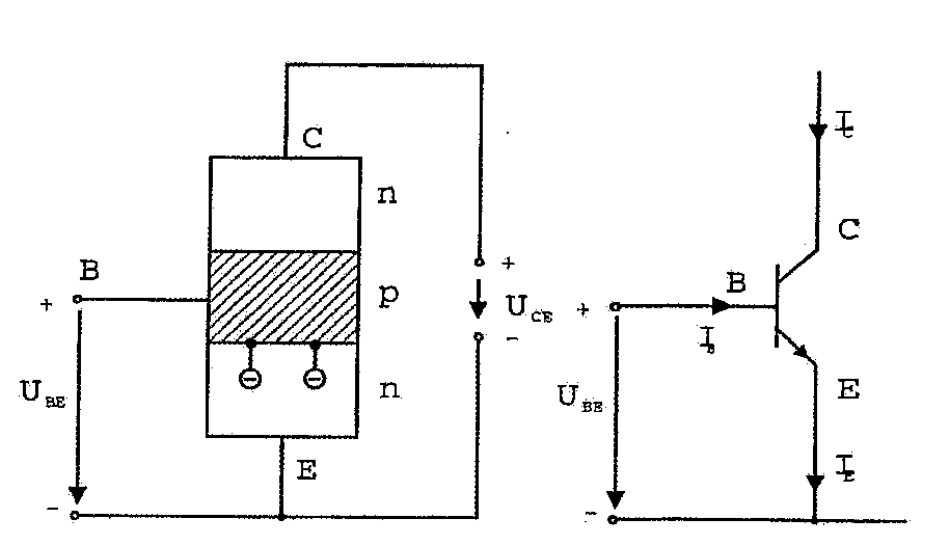
\includegraphics[width=0.66\textwidth]{fig/npn-transistor}
        \caption{NPN Bipolar Transistor}
        \label{fig:transistor-npn}
    \end{figure}
    
    \begin{figure}
        \centering
        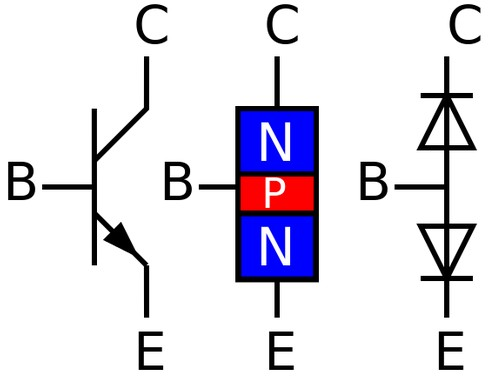
\includegraphics[width=0.33\textwidth]{fig/transistor-npn-diode.jpg}
        \caption{NPN Transistor und sein Diodenersatzschaltbild.}
        \label{fig:transistor-npn-diode}
    \end{figure}
    
    \begin{figure}
        \centering
        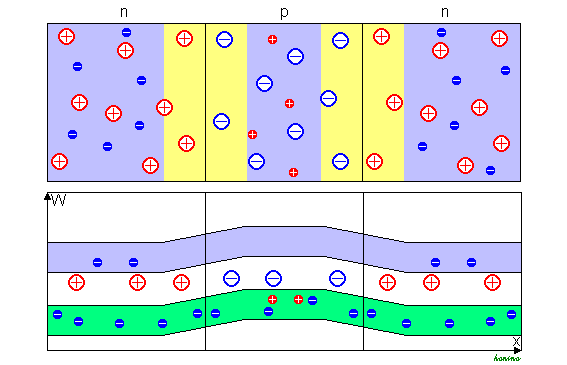
\includegraphics[width=0.33\textwidth]{fig/npn-bipolartransistor-band1.PNG}\hfill
        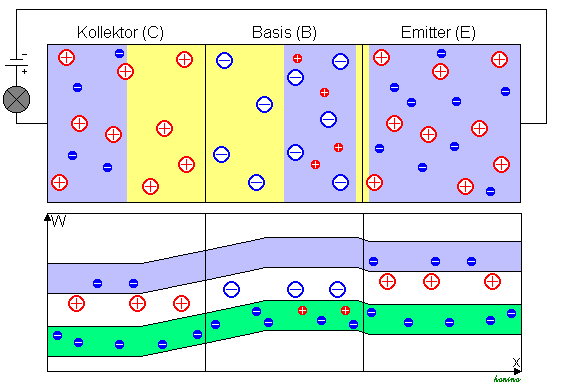
\includegraphics[width=0.33\textwidth]{fig/npn-bipolartransistor-band2.PNG}\hfill
        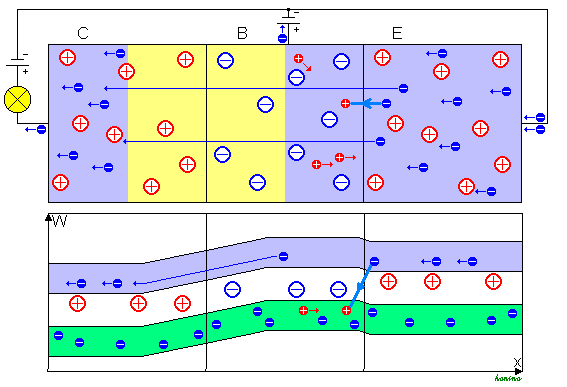
\includegraphics[width=0.33\textwidth]{fig/npn-bipolartransistor-band3.PNG}
        \caption{\textbf{Links:} Kristallaufbau und Bändermodell eines Bipolartransistors. \textbf{Mitte:} Selbiges bei angelegter Kollektor-Emitter Spannung. \textbf{Rechts:} Zusätzlich mit angelegter Basis-Emitter Spannung.}
        \label{fig:npnTransistor}
    \end{figure}
    
    \subsubsection{Physikalischer Aufbau}
    Ein Bipolartransistor besteht aus drei dünnen Halbleiterschichten, die übereinander gelegt sind. Die mittlere Schicht ist im Vergleich zu den zwei äußeren Schichten sehr dünn.
    
    \subsubsection{Funktionionsweise}
    Durch einen kleinen elektrischen Strom $I_B$ an der Basis wird ein größerer Strom $I_C$ zwischen Kollektor und Emitter gesteuert. 
   
   \begin{enumerate}
    \item \emph{Aktive Kollektor-Emitter Spannug $U_{CE} > 0$:} Wird nur eine Spannung zwischen Kollektor und Emitter angelegt ($U_{CE} > 0$), entspricht das Schaltungstechnisch einfach zwei entgegengesetzten Dioden, von denen eine immer gesperrt ist (Für npn ist das die Basis Kollektor Diode). 
    Die angelegte Spannung verringert zwar die Basis-Emitter Sperrschicht, die Basis-Kollektor Sperrschicht (auch Raumladungszone) vergrößert sich aber gleichzeitig.  
    
    \item \emph{Zuschaltung von $U_{BE} > 0.7$:} Wird nun zusätzlich eine Basis Emitter Spannung von mehr als 0.7V angelegt, dann werden Elektronen aus dem Emitter in die Basis injiziert. Diese Elektronen rekombinieren prinizpiell mit den Löchern in der Basis. Da die Basis aber sehr, sehr klein ist, diffundieren mehr als 99\% der Elektronen in die Basis-Kollektor Sperrschicht. Da bereits eine Spannung $U_{CE} > 0$ anliegt, wandern die Elektronen durch die Potentialdifferenz gleich weiter aus dem Kollektor hinaus. Dieser vom Emitter zum Kollektor fließende Storm ist dann $I_C$.
    
    
    \item \emph{Durchlass (anders formuliert, sonst wie 2:} Wird eine Spannung $U_{BE} > 0.7V$ zwischen Basis und Emitter angelegt, dann kann das elektrische Feld der Raumladungszone von Elektronen überwunden werden.
    Dabei gelangen die Elektronen von der n-Schicht des Emitters in die p-Schicht der Basis und können von dort aus der Basis hinaus fließen, da sie von der positiven Seite der Spannungsquelle (die auch $U_{BE}$ erzeugt) angezogen werden.
    Da aber die p-Schicht so klein ist, können nicht alle Elektronen über die Basis abfließen sondern wandern weiter in die obere Grenzschicht.
    
    Die vom Emitter in die Basis injizierten Elektronen werden von der Basis-Collector Raumladungszone abgesaugt und fließen \textit{nicht} über den Basisanschluss. 
   \end{enumerate} 
    
    
    \subsubsection{Skizze}
    
    \begin{figure}
        \centering
        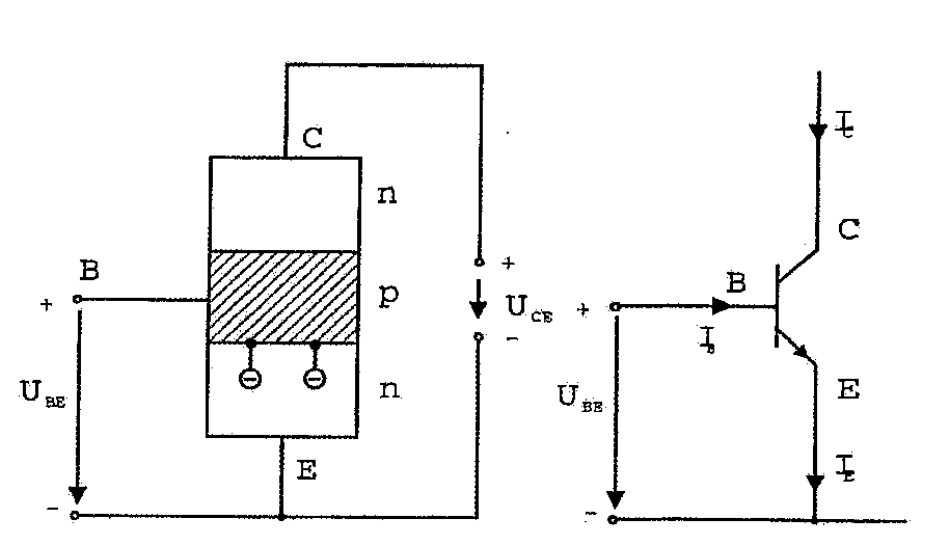
\includegraphics[width=0.66\textwidth]{fig/npn-transistor.jpg}
        \caption{Schematischer Aufbau und Schaltsymbol des npn-Transistors}
        \label{fig:npnTransistor}
    \end{figure}
    
    \begin{figure}
        \centering
        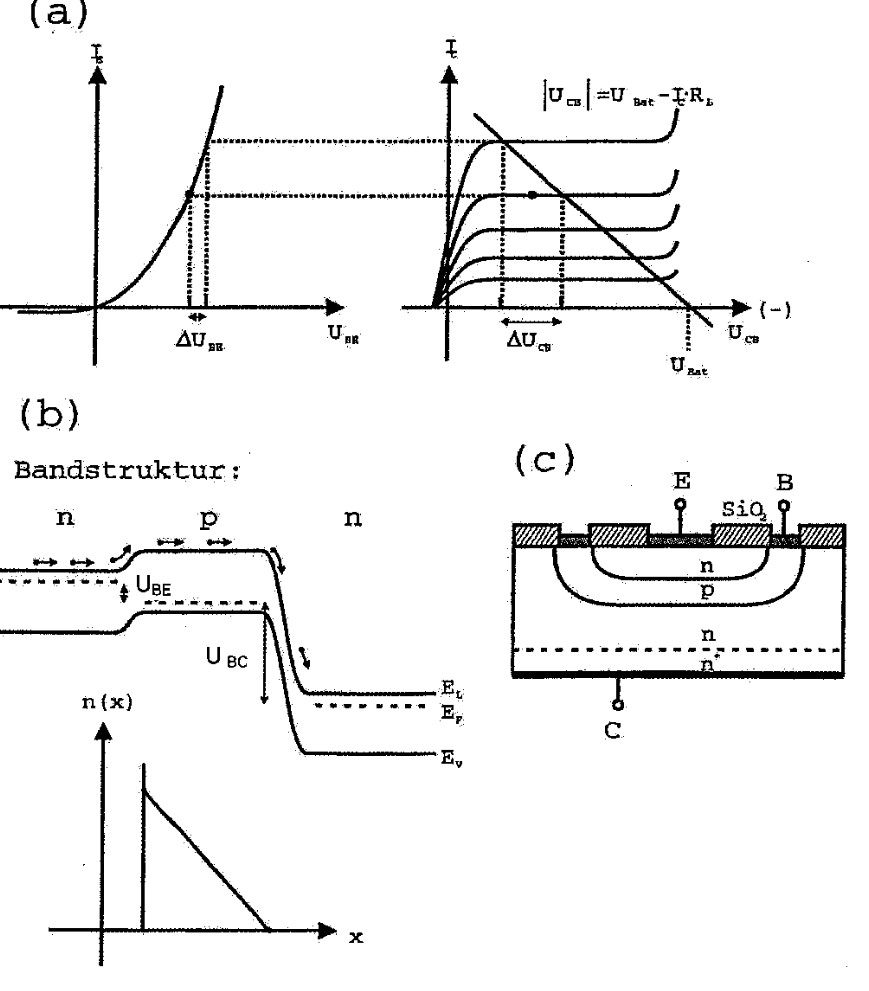
\includegraphics[width=0.66\textwidth]{fig/npn-transistor-kennlinien.jpg}
        \caption{Transistor - eine Hintereinanderschaltung zweier Dioden. Steile EB-Durchlasskennlinie steuer hochohmige EC-Diode. Weiters sind die Bandstruktur im Ort, der schematische AUfbau und das Diffusionsdreieck dargestellt.}
        \label{fig:npnTransistorKennlinie}
    \end{figure}
    
    \subsubsection{Warum wird er als Verst\"arker eingesetzt?}
     
    
\subsection{MOS-Struktur und Inversion \todo{2x}}\label{k6:mosInversion}

    \subsubsection{Wann spricht man von Inversion}
    Von MOS-Inversion spricht man, wenn sich die Ladungsträgerdichten in einem Halbleiter lokal ändern und er seine Eigenschaften aus dem Grundzustand "verliert".
    
    \emph{Exakte Definition:} Die Inversion ist dann erreicht, wenn die Zahl der Elektronen an der Oberfläche gleich groß ist, wie die Zahl der Löcher im Volumen des Halbleiters. Diese Situation ist dann gegeben, wenn die Bandverbiegung $\Phi_S = 2\Phi_F$ ist.Die äußere Spannung die dazu notwendig ist, wird dementsprechend auch Schwellwertspannung (Thresholdvoltage) genannt. \autoref{fig:mos-energie} zeigt die Energieniveaus.
    
    \begin{figure}
        \centering
        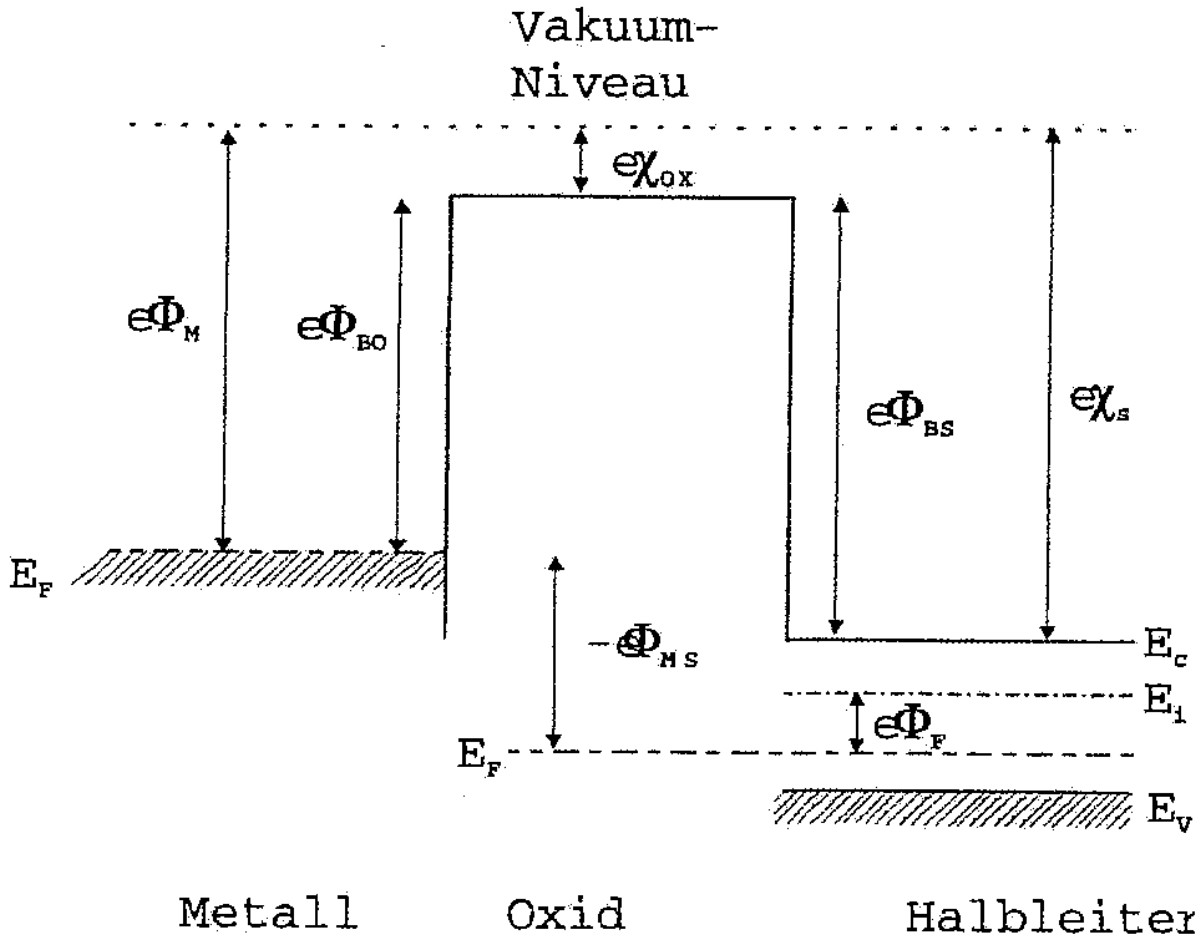
\includegraphics[width=0.66\textwidth]{fig/mos-energie.jpg}
        \caption{Energetische Verhältnisse in einer Metall-Oxid Halbleiter-Struktur unter Flachband-Bedingungen. }
        \label{fig:my_label}
    \end{figure}
    
    \emph{Beispiel P-MOS: \autoref{fig:mos-inversion2}}
    \begin{enumerate}
        \item Der Halbleiter ist p-dotiert, d.h. es gibt mehr Löcher als Elektronen.
        \item Am Gate wird eine negative Spannung angelegt, d.h. die Dichte an Löchern erhöht sich dort und es entsteht ein starker Potentialgradient zum Halbleiter.
        \item Alle freien Elektronen des Halbleiters wandern in Richtung des Gates um den Gradient wieder auszugleichen.
        \item Entlang des Gates entsteht eine Zone mit mehr freien Elektronen als Löchern. Lokal betrachtet verhält sich der Halbleiter hier also eher wie ein n-dotierter Halbleiter, nicht wie ein p-dotierter. Daher der Name \textbf{MOS-Inversion}.
    \end{enumerate}
    
    \begin{figure}[H]
        \centering
        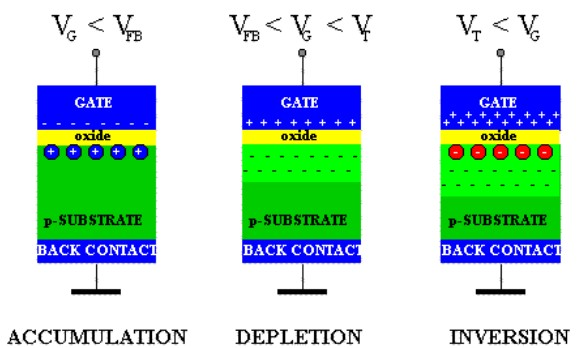
\includegraphics[width=0.33\textwidth]{fig/mos-inversion.jpg}
        \caption{Ganz rechts: Die Inversion in einem MOS mit p-Substrat.}
        \label{fig:mos-inversion2}
    \end{figure}
    
    \subsubsection{Leitungsband, Valenzband, Ef aufzeichnen}

\subsection{Diffusions-Dreieck beim Transistor \todo{0x}}\label{k6:diffusionsdreieck}

\autoref{fig:npnTransistorKennlinie}
    \subsubsection{Warum fast linear?} exponential-Funktion im Ursprung ann\"ahernd linear
    \subsubsection{Was w\"are wenn die Basisl\"ange gr\"o{\ss}er als die Diffusionsl\"ange w\"are?} Man h\"atte die Wirkung von 2 Dioden und keinen Transistoreffekt mehr.

\subsection{Feldeffekt-Transistor \todo{0x}}\label{k6:fet}


\subsection{MOS-FET \todo{0x}}\label{k6:mosfet}

Bipolartransistor kann man sich als 2 Schleusen vorstellen, wobei eine kleine Schleuse über einen Hebel die größere Steuert. 
MOS-FET kann man sich als Wasserschlauch vorstellen, bei dem man von außen drauf treten kann um den Fluss zu regulieren.
Daran kann man relativ schnell erkennen, dass ein MOS-FET a.) weniger Strom braucht und b.) schneller schaltet als ein Bipolartransistor. 

Die wichtigsten Begriffe in einem MOS-System sind Akkumulation, Verarmung und Inversion.
Diese Breiche sind quantitativ über die Flachbandspannung $V_FB$ (Die externe Spannung, zur der es im Halbleiter keine Bandverschiebung gibt) definiert. 
Hier kurz für p-dotiertes Silizium:
\begin{enumerate}
    \item Akkumulationsbereich ($V_G \ll V_{FB}$): Hauptsächlich Majoritätsladungsträger (Löcher) unter der Gate Elektrode (\autoref{fig:mos-akkumulation})
    \item Verarumungsbereich ($V_G > V_{FB}$): WEniger Majoritätsladungsträger (Löcher) unter der Gate-Elektrode als normal (\autoref{fig:mos-verarmung}) 
    \item Inversionbereich ($V_G \gg V_{FB}$): Es sammeln sich Minoritätsladungsträger (Elektronen) unter dem Gate. (\autoref{fig:mos-inversion}) 
\end{enumerate}

    \begin{figure}[H]
        \centering
        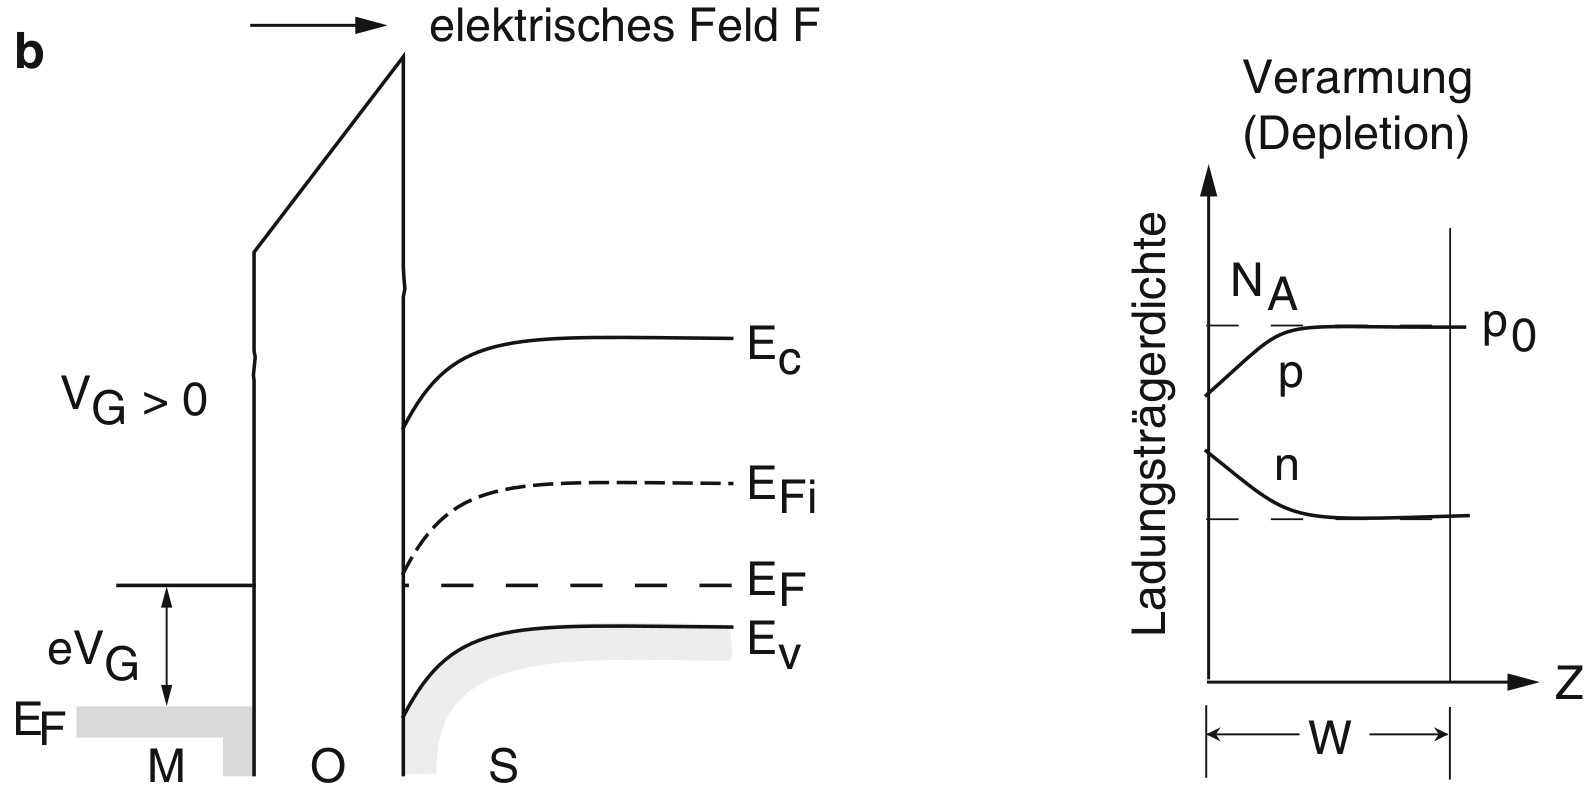
\includegraphics[width=0.66\textwidth]{fig/mos-verarmung}
        \caption{MOS Band-Diagramm und Ladungsträgerdichte für Verarmung.}
        \label{fig:mos-verarmung}
    \end{figure}
    \begin{figure}[H]
        \centering
        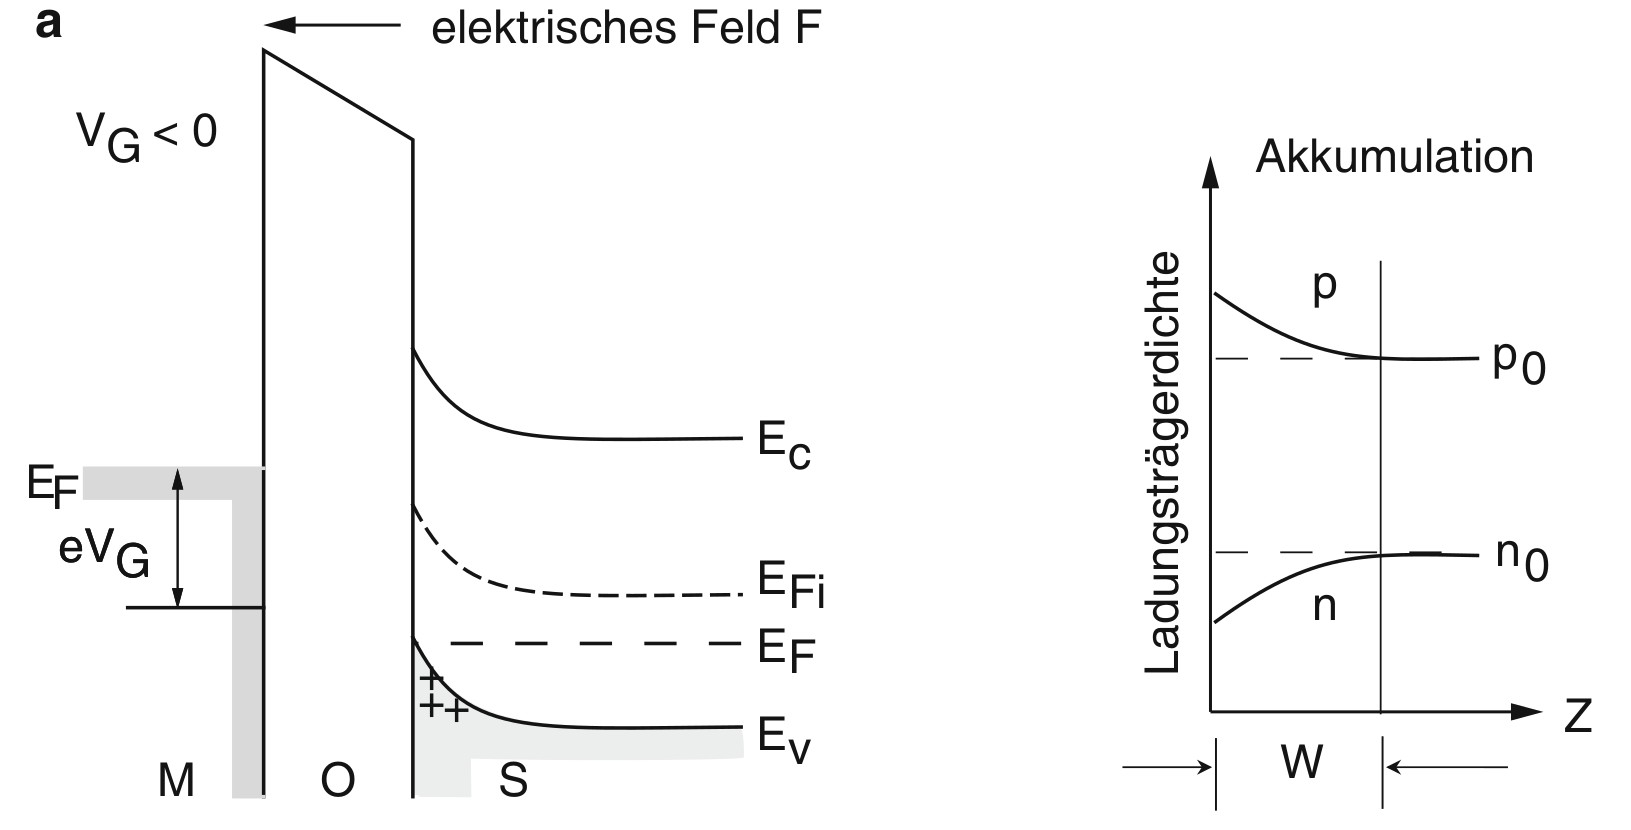
\includegraphics[width=0.66\textwidth]{fig/mos-akkumulation}
        \caption{MOS Band-Diagramm und Ladungsträgerdichte für Akkumulation.}
        \label{fig:mos-akkumulation}
    \end{figure}
    \begin{figure}[H]
        \centering
        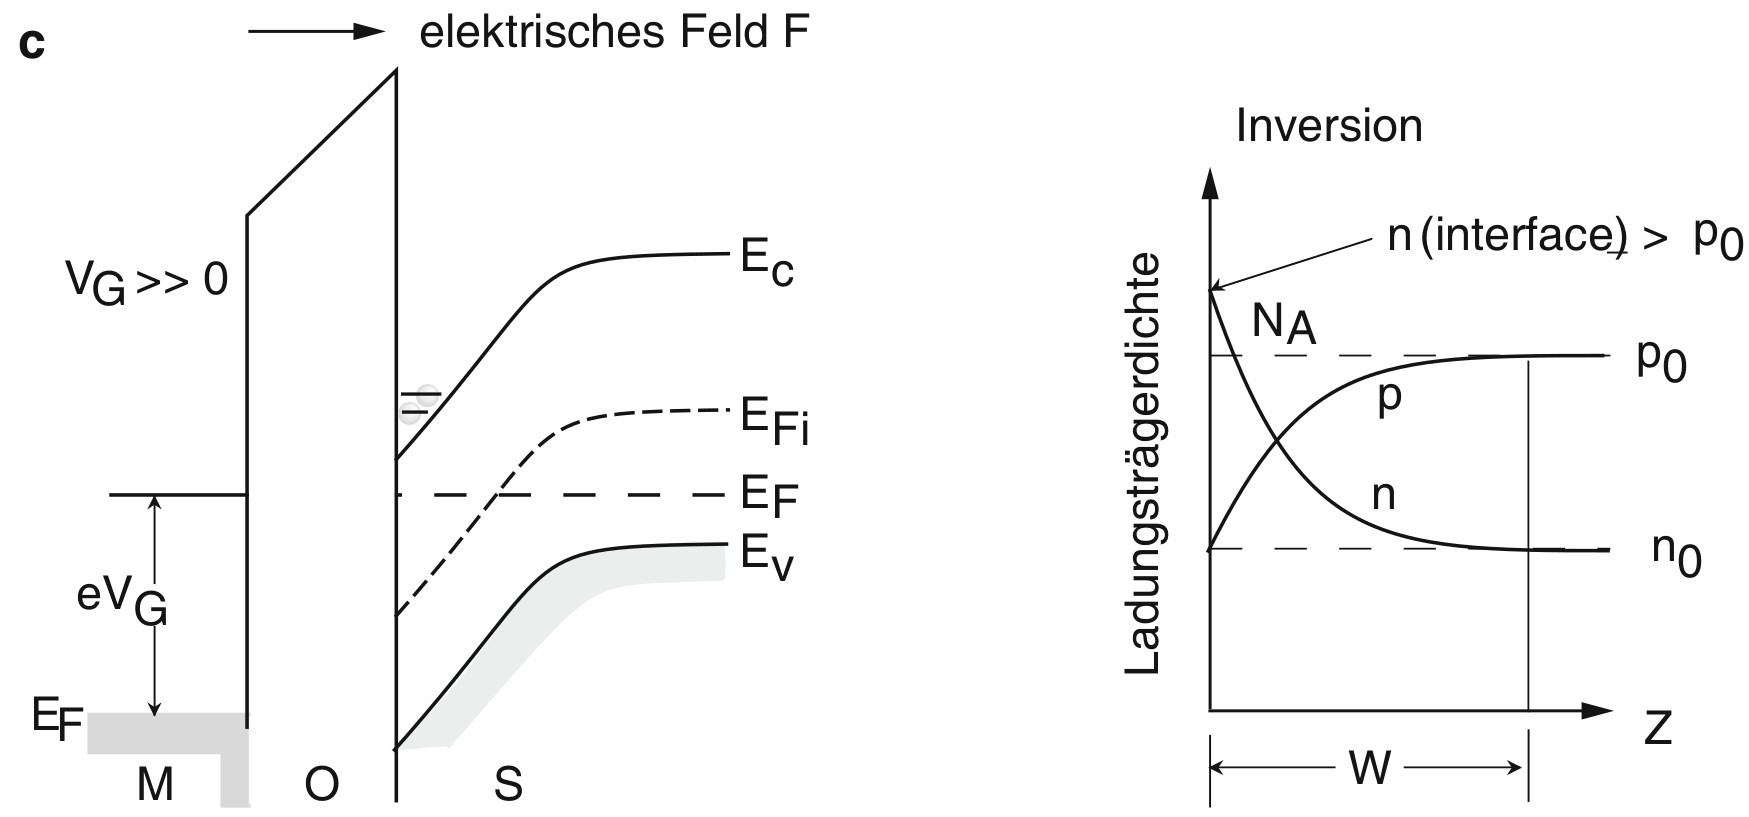
\includegraphics[width=0.66\textwidth]{fig/mosfet-inversion}
        \caption{MOS Band-Diagramm und Ladungsträgerdichte für Inversion.}
        \label{fig:mos-inversion}
    \end{figure}

    \subsubsection{Aufbau}
    Siehe \autoref{fig:mos-aufbau}, \autoref{fig:mos-aufbau2}.
    \begin{figure}[H]
        \centering
        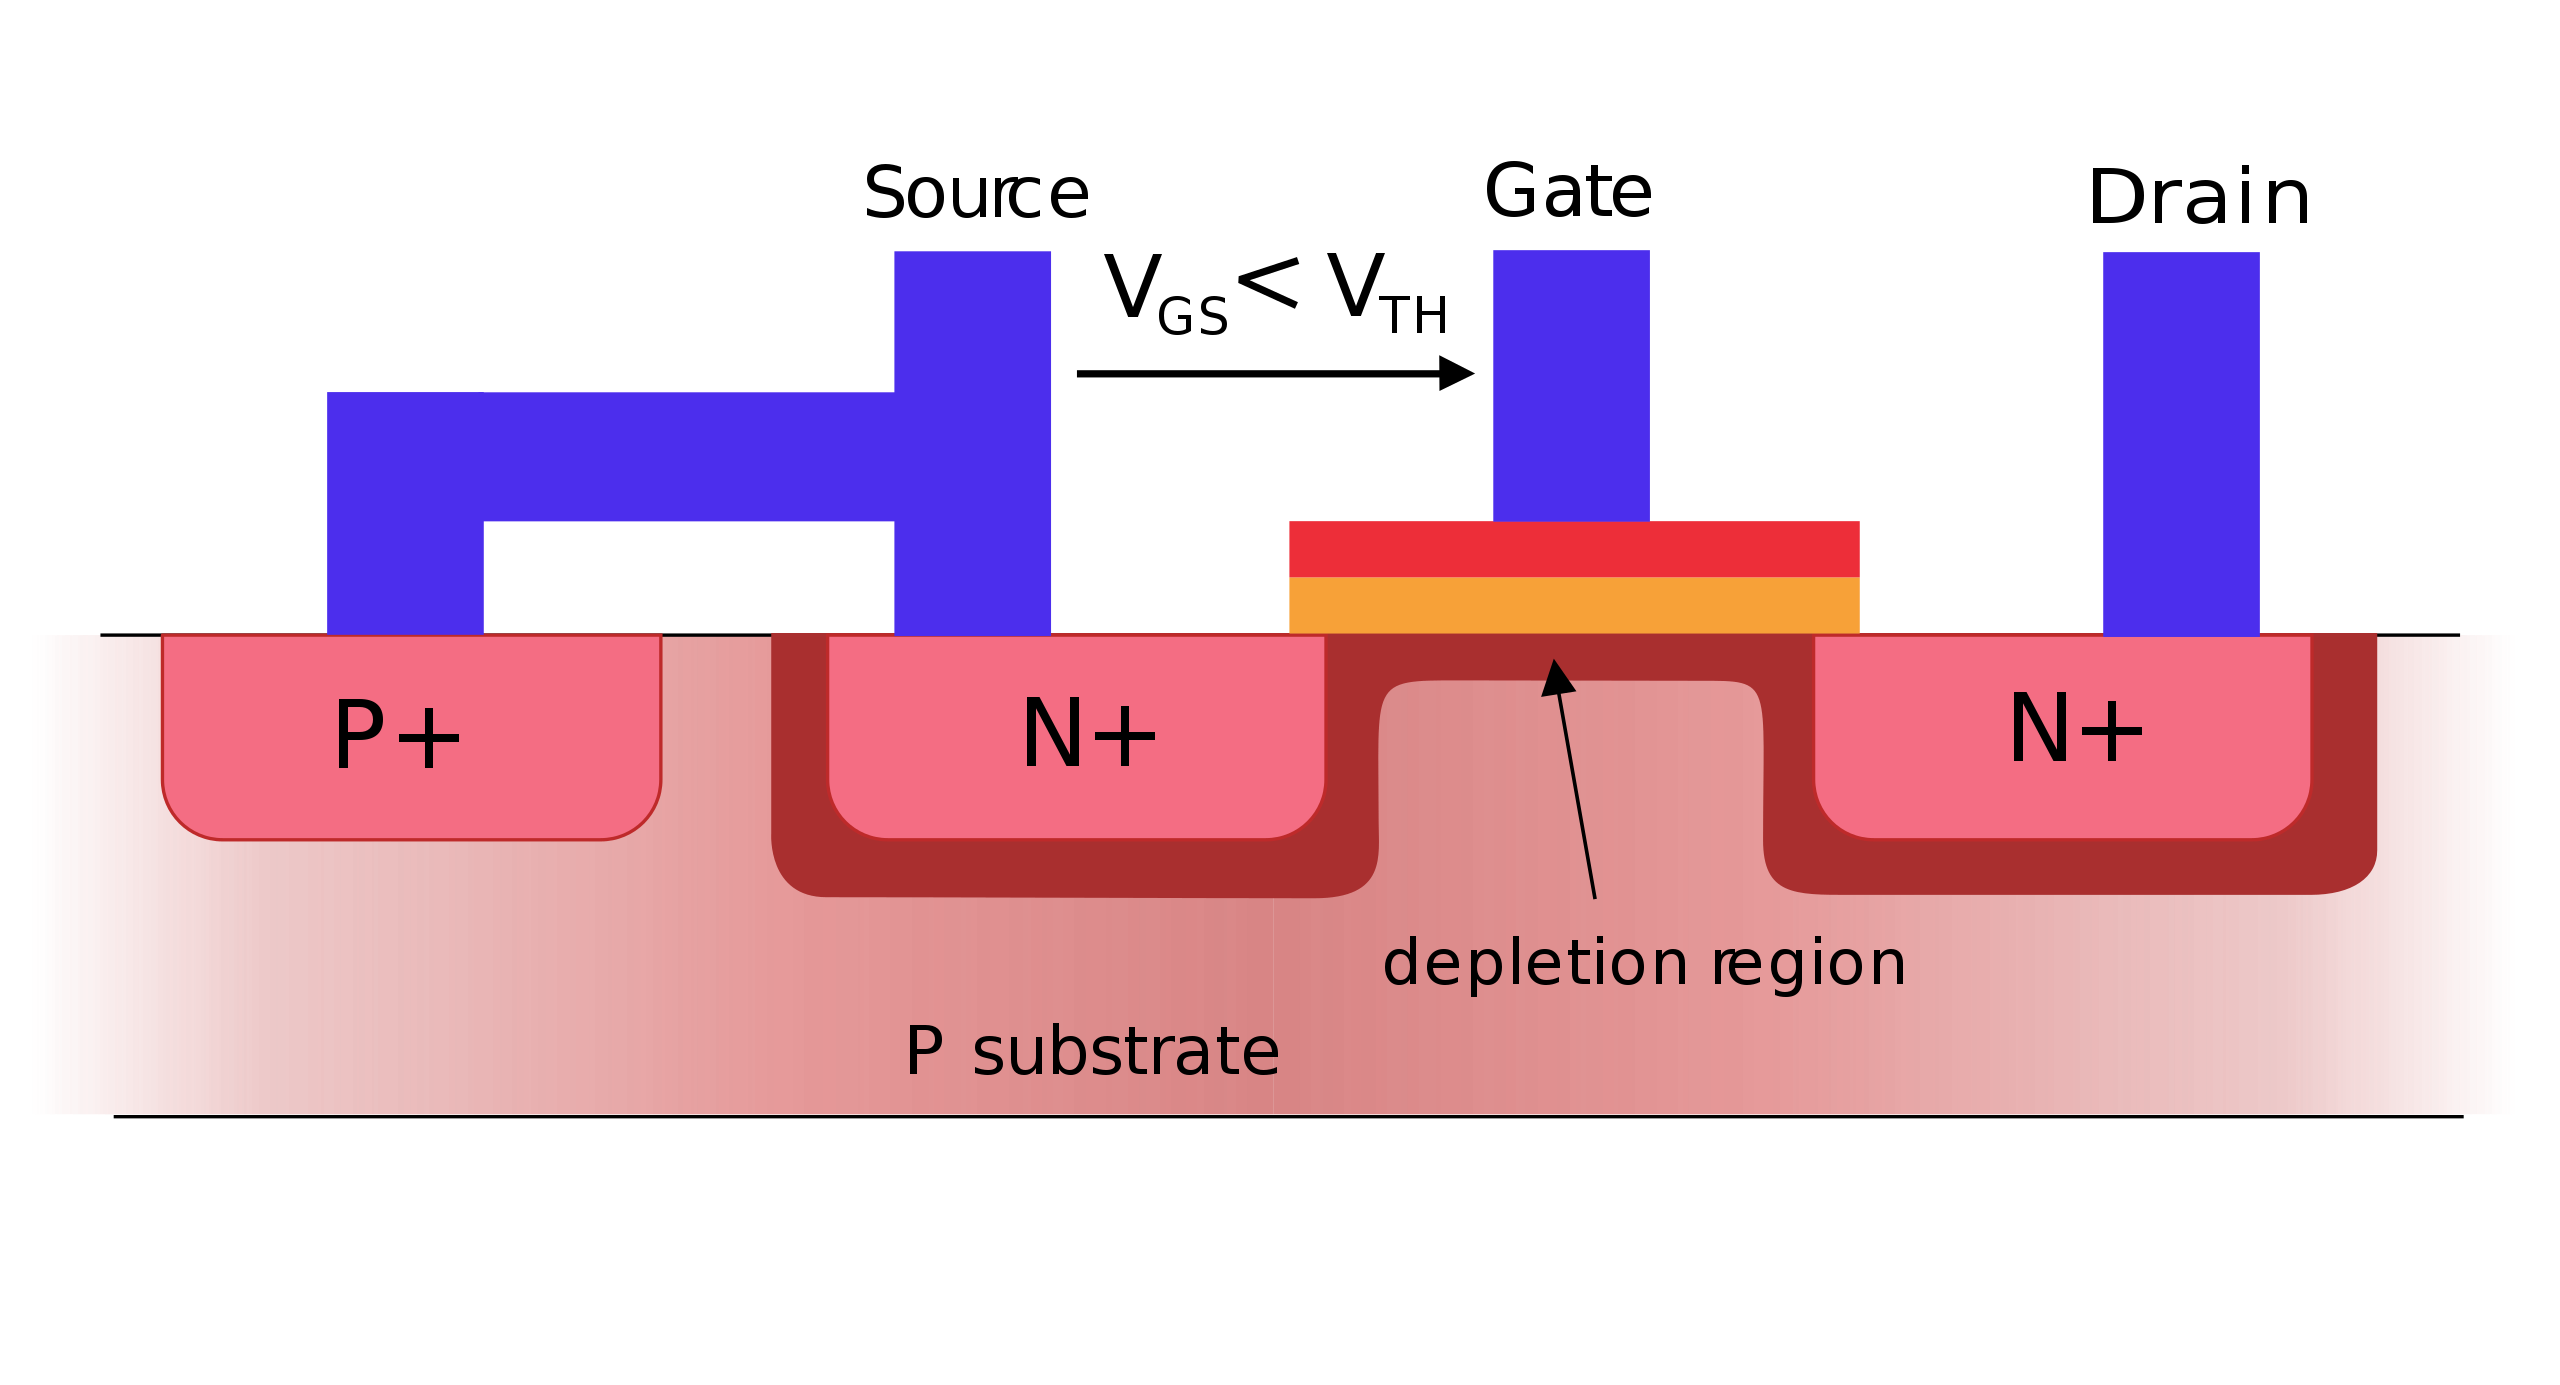
\includegraphics[width=0.66\textwidth]{fig/mos-aufbau.png}
        \caption{A cross-section through an nMOSFET when the gate voltage VGS is below the threshold for making a conductive channel; there is little or no conduction between the terminals drain and source; the switch is off. When the gate is more positive, it attracts electrons, inducing an n-type conductive channel in the substrate below the oxide, which allows electrons to flow between the n-doped terminals; the switch is on.}
        \label{fig:mos-aufbau}
    \end{figure}
    
    \begin{figure}[H]
        \centering
        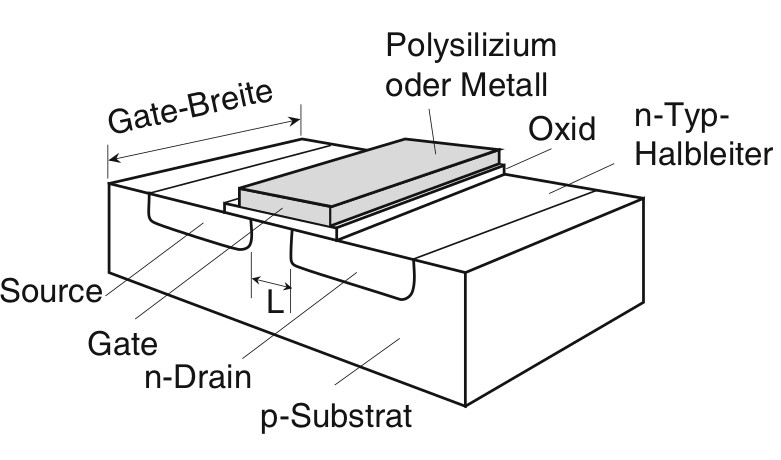
\includegraphics[width=0.66\textwidth]{fig/mos-aufbau2}
        \caption{Nochmal der Aufbau eines MOSFETs.}
        \label{fig:mos-aufbau2}
    \end{figure}
    
    \subsubsection{Flachband und Inversion}
    Wird eine Spannung am Gate angelegt (für p-MOS), dann werden die Löcher in das innere des Halbleiters verschoben (Also vom Gate weg). Es entsteht also eine \textit{Verarmungszone}, in der Elektronen dominieren. Diese Verarmungszone kann man wie eine Raumladungszone betrachten - es gibt keine leitende Verbindung zwischen Source und Drain.
    
    Erreicht die Gatespannung aber den Schwellwert $U_T$ (Thresholdspannung), dann bildet sich an der Halbleiteroberfläche eine sogenannte \textit{Inversionsschicht} aus, in der Elektronenleitung auftritt. Damit besteht eine leitende Verbindung zwischen Source und Drain, der sogenannte \textit{Kanal}. 
    
    Im \textit{Flachbandfall} ist die Löcherdichte an der Grenzfläche exakt gleich wie im Inneren des Substrates. Wird die Bandverbiegung so groß, dass das Leitungsband an der Grenzfläche dem Ferminiveau nahe kommt, treten an der Grenzfläche Elektronen auf. 
    
    
    \subsubsection{Bandstruktur}
    
    \begin{figure}
        \centering
        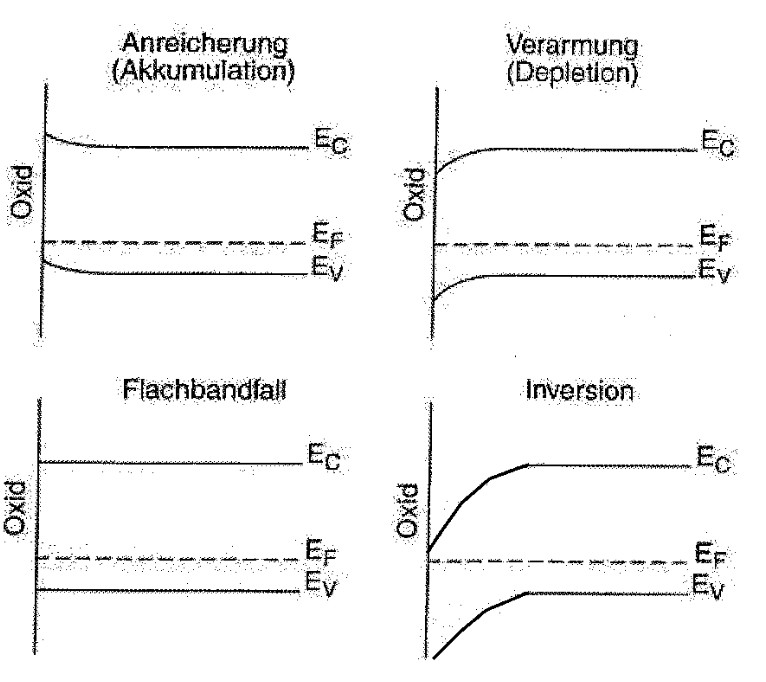
\includegraphics[width=0.66\textwidth]{fig/mos-bänder2.jpg}
        \caption{Bandschema des MOSFET normal zur Oberfläche für verschiedene Gatespannungen. 
        Links ist immer das Oxid eingezeichnet, das Band entfernt sich dann weg vom Oxid. Akkumulation, Verarmung, FLachbandfall, Inversion.}
        \label{fig:mos-bänder2}
    \end{figure}
    
    
    \begin{figure}
        \centering
        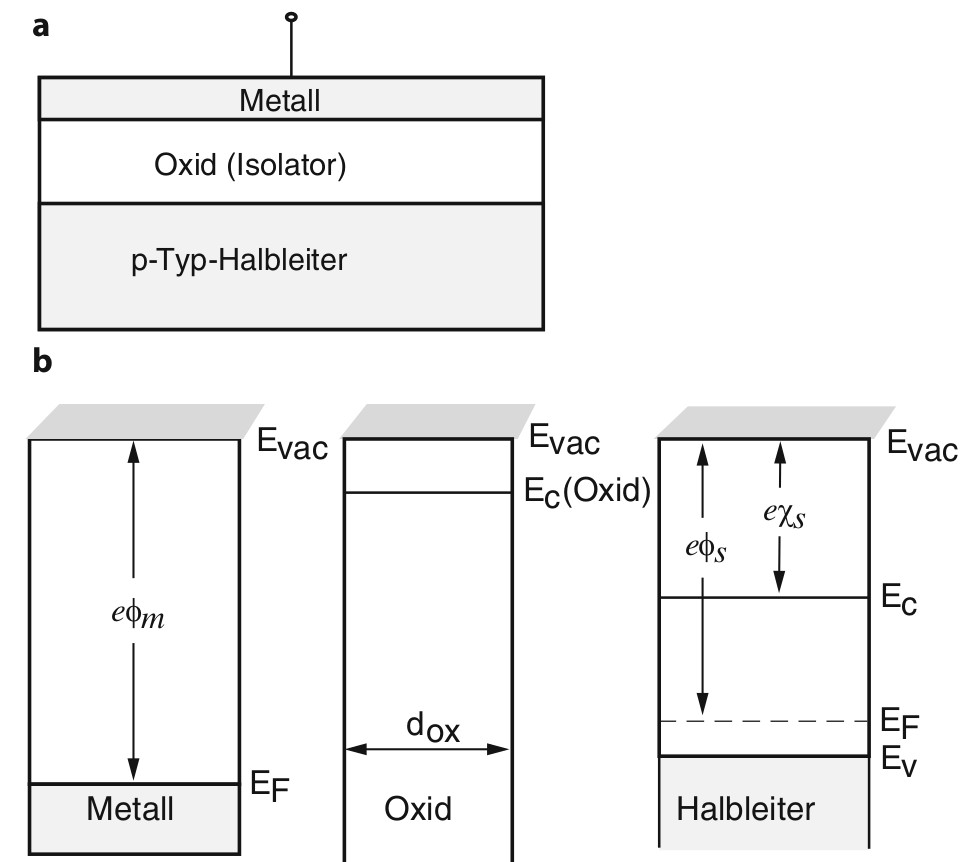
\includegraphics[width=0.66\textwidth]{fig/mos-bänder1.jpg}
        \caption{(a) Aufbau einer MOS-Struktur. (b) Austrittsarbeiten, Nadlücken, Fermi-Niveaus etc. in einem Metall, einem Oxi und einem Halbleiter}
        \label{fig:mos-bänder1}
    \end{figure}
    
    \begin{enumerate}
        \item $\Phi_S$: Austrittsarbeit (Abstand vom Fermi-Niveau zum Vakuum) im Halbleiter
        \item $\Xi$ Energieabstand zwischen Leitungsband un dVakuum
        \item $\Phi_B^n = \frac{kT}{e}ln(\frac{N_D}{n_i})$: Abstand zwischen Fermi-Niveau und Leitungsband im n-Typ-Halbleiter
        \item $\Psi(z) = \Phi(z) - \Phi_B$ Bandverbiegung
        \item $V_{FB}$: Flachbandspannung: Extern angelegte Spannung, bei der es keine Bandverbiegungen im Halbleiter gibt. 
        \item $\omega = \sqrt{\frac{2*\Psi_S \epsilon_S}{eN_A}}$: Breite der Verarmungszone (depletion zone) im Halbleiter, hier für das p-Typ-Silizium
    \end{enumerate}
    
    \begin{figure}
        \centering
        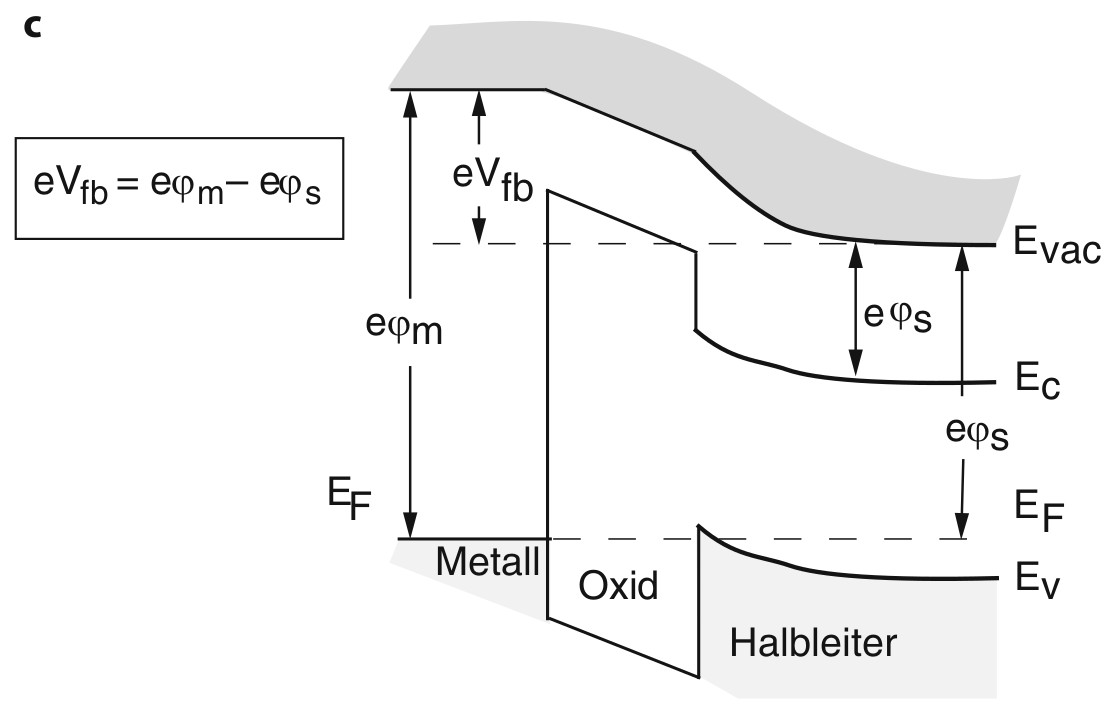
\includegraphics[width=0.66\textwidth]{fig/mos-leitungsband.jpg}
        \caption{Leitungsbandprofil der fertigen MOS-Struktur.}
        \label{fig:mos-bänder}
    \end{figure}
    

\subsection{MES-FET \todo{0x}}\label{k6:mesfet}

\subsection{Early-Effekt \todo{0x}}\label{k6:early}
Eine kleine Abhängigkeit des Kollektorstromes von $U_{CB}$ wird durch den sogenannten
Early-Effekt verursacht. Eine höhere Sperrspannung $U_{CB}$ bewirkt eine wachsende RLZ
zwischen C und B. Der rechte Rand der neutralen Basiszone wandert somit etwas nach
links, der Effektivwert von W wird kleiner, das Diffusionsdreieck steiler und $I_C$ größer.
Bei sehr großem $U_{CB}$ frisst die RLZ die gesamte Basis auf: Dieser Punch-through-Effekt
stellt eine Grenze für $U_{CB}$ dar.

\begin{enumerate}
    \item \emph{Ursache:} Wird die Kollektor-Emitter Spannung erhöht, dann vergrößert sich die Raumladungszone des Kollektor-Basis Übergangs und die Weite der Basis verringert sich.
    \item \emph{Auswirkung:} Der Transistor ist keine ideale Stromquelle, da der Kollektorstrom von der Kollektor-Emitter Spannung $U_{CE}$ abhängt.
    \item \emph{Größenordnung:} Liegt bei Transistoren betragsmäßig zwischen 15V und 150V. 
\end{enumerate}

Eine verkleinerte Basis hat zur folge, dass Elektronen mit einer geringeren Wahrscheinlichkeit in der Basis rekombinieren.
Daraus folgend müssen mehr Elektronen über den Kollektor fließen, der Strom erhöht sich in einer nicht-linearen Art und Weise. 

    \begin{figure}
        \centering
        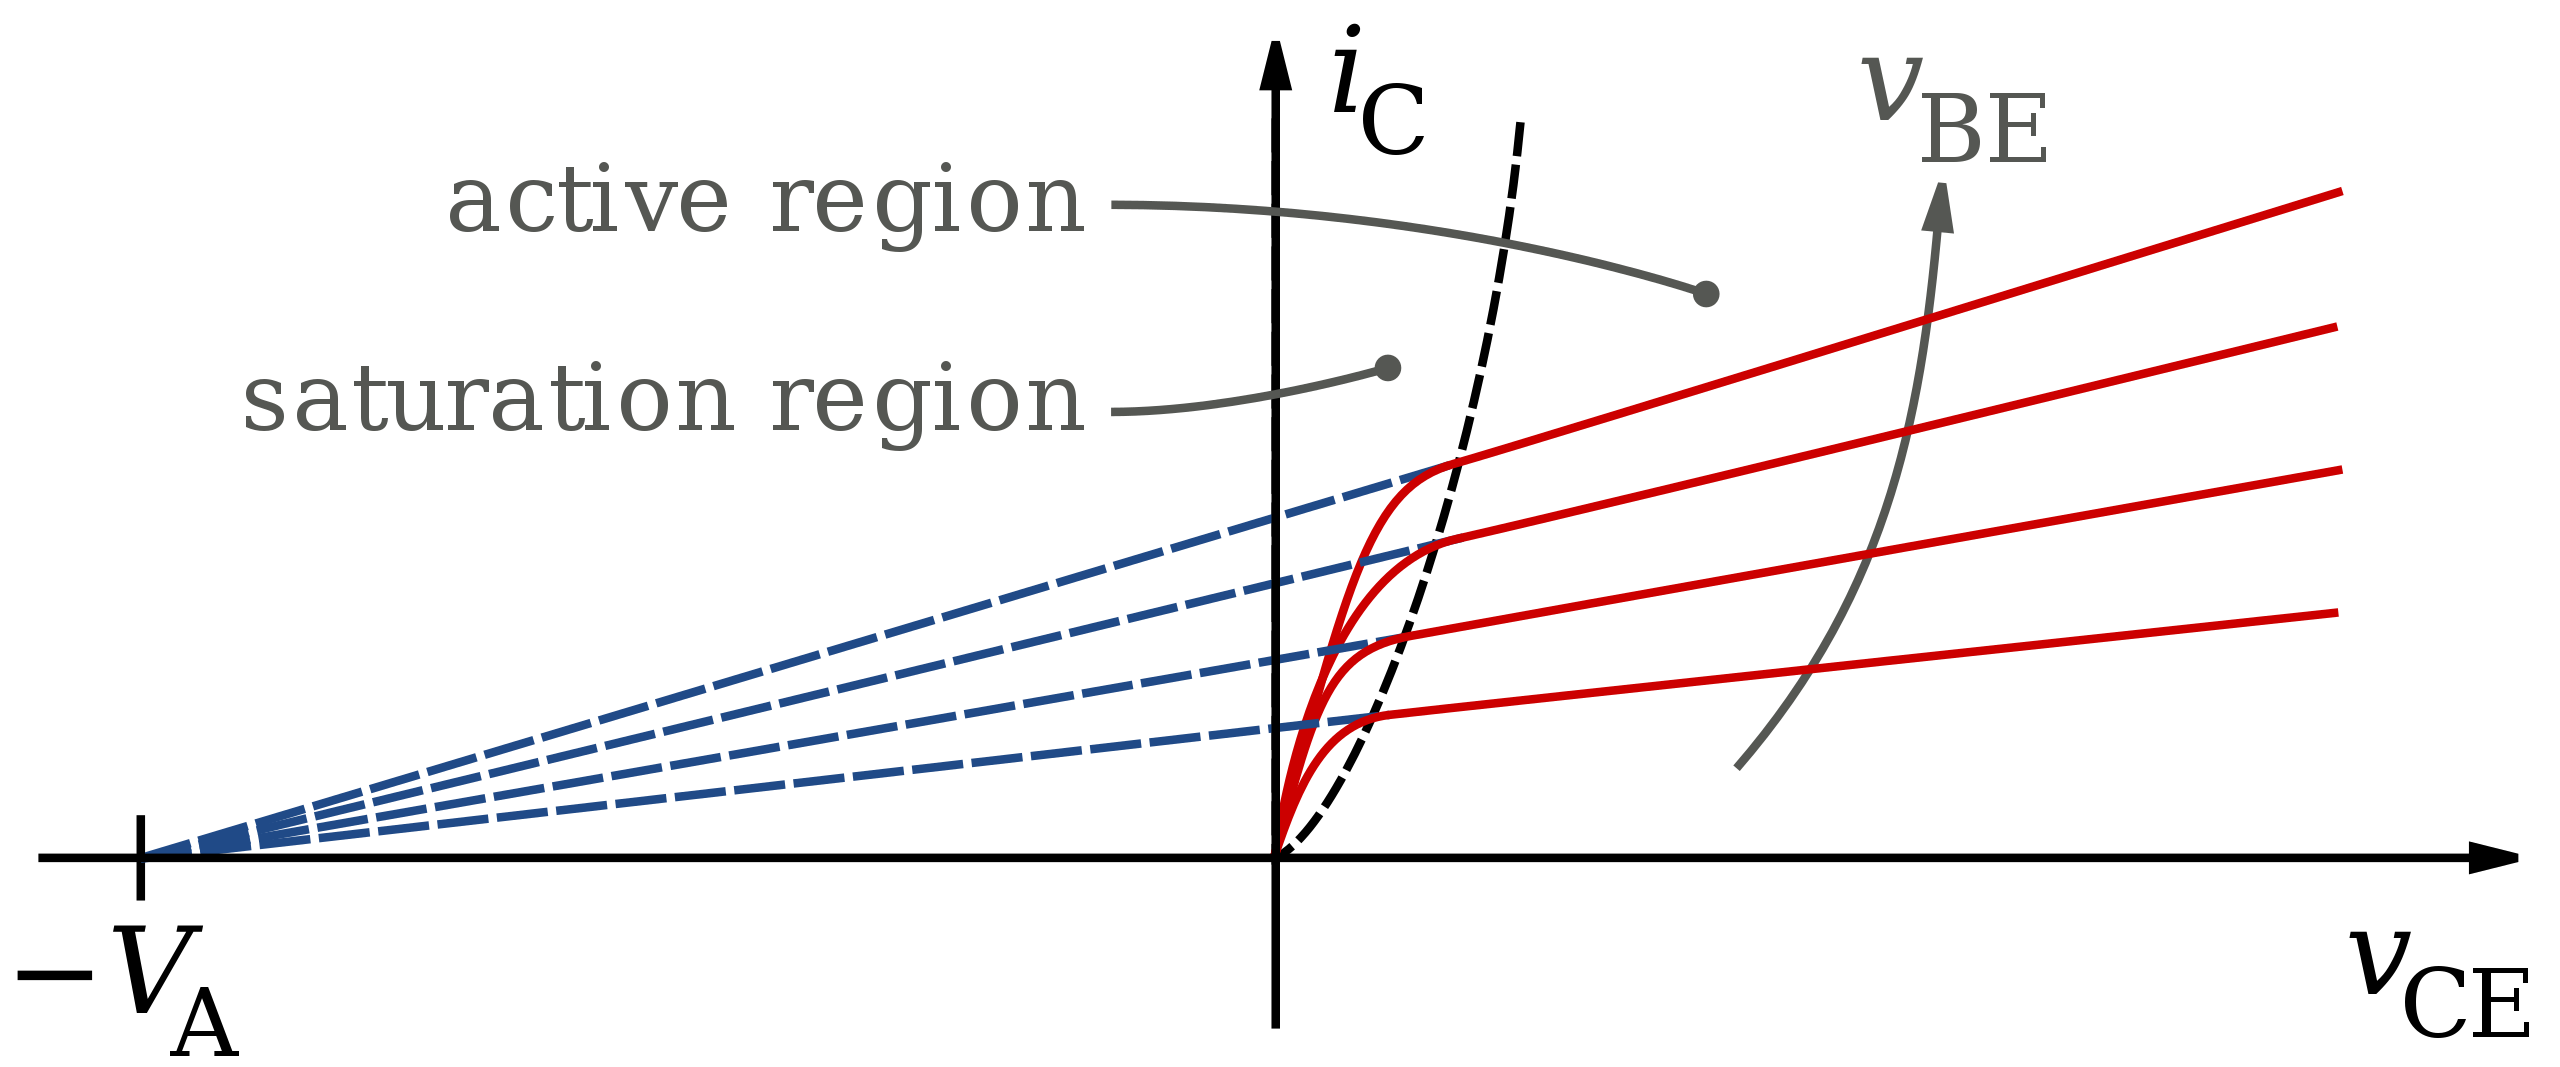
\includegraphics[width=0.66\textwidth]{fig/transistor-early-effect.png}
        \caption{Early-Spannung ist der Punkt ganz links}
        \label{fig:npnTransistorKennlinie}
    \end{figure}


\subsection{JFET \todo{0x}}\label{k6:jfet}

    \begin{figure}[H]
        \centering
        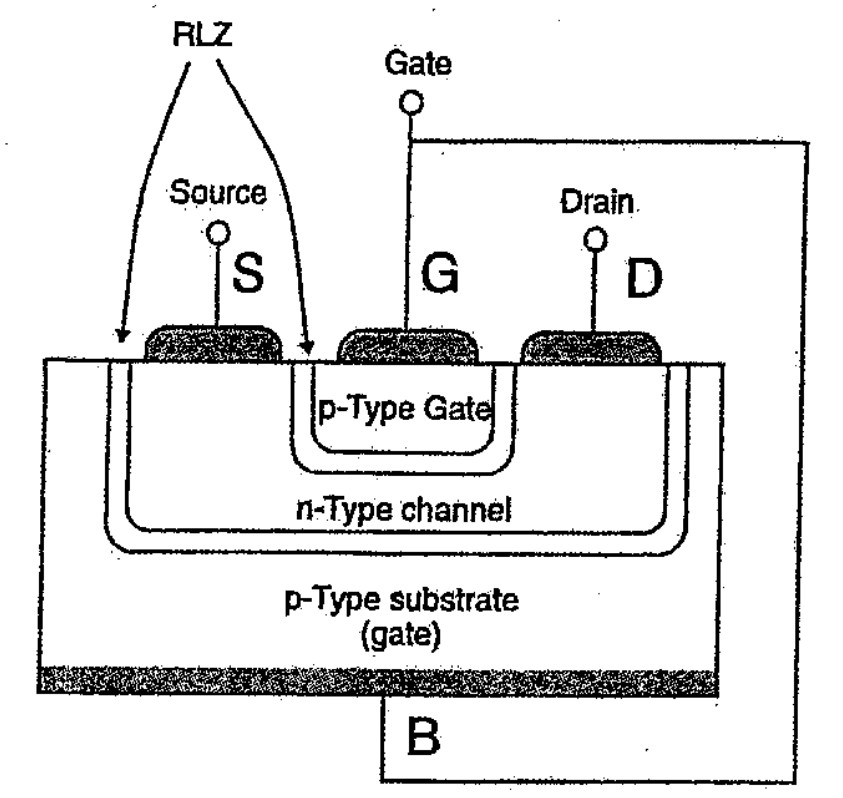
\includegraphics[width=0.66\textwidth]{fig/jfet-aufbau.jpg}
        \caption{Aufbau eines Sperrschichtfeldeffekt Transistors (JFET - \textbf{J}unction \textbf{F}ield \textbf{E}ffect \textbf{T}ransistor)}
        \label{fig:jfet-aufbau}
    \end{figure}

In \autoref{fig:jfet-aufbau} ist der Aufbau eines n-Kanal Sperrschicht-Feld Effekt Transistors zu sehen. 

Im Transistor befindet sich ein n-leitender Kanal, durch den Elektronen von der Source Elektrode S zur Drain Elektrode D fließen können, wenn $U_{DS} > 0$ ist (Drain-Source Spannung).

Die steuernde Gate Elektrode G ist leitend mit einer p-dotierten Zone verbunden, die durch eine Sperrschicht vom Kanal getrennt ist. 
Für $U_{GS} > 0$ ist dieser pn-Übergang in Sperrichtung gepolt.

\subsubsection{JFET vs MOSFET}
JFET und MOSFET haben nahezu identische Eigenschaften. Abgesehen von den verschiedenen Herstellungsverfahren ist als Unterschied hervorzuheben, dass für den JFET nu rjene Polarität von $U_{GS} $ verwendet werden darf, für die das Gate-Gebiet gegen den Kanal in Sperrrichtung gepolt ist. 

\subsubsection{FET vs Bipolar-Transistor}

\textbf{Vorteile FET}
\begin{enumerate}
    \item Sehr kleiner Gatestrom bei Gleichspannung (MOSFET $I_G < ipA$)
    \item Im Schalterbetrieb müssen keine Speicherladungen abgeführt werden. 
    \item Die Schwellspannung kann in weiten Grenzen bei der Herstellung eingestellt werden.
    \item Leichte Integrierbarkeit des MOSFET (nicht für JFET). Weit weniger verschiedene Diffusionsprozesse und photolithographische Prozesse bei der Herstellung nötig und der Platzbedarf ist geringer.
    \item Geringes Rauschen
    \item Keine Offset Spannung bei Zerhacker Anwendungen, weil sich im eingeschalteten Zustand der Kanal wie ein ohmscher Widerstand verhält, d.h. $I_D=0$ für $U_{DS} = 0$
    \item Unempfindlicher gegenüber Strahlungsschäden
    \item Schwächere Temperaturabhängigkeit. Im Bipolar ist die Minoritätendichte wesentlich, die proportional zu $n_i^2$ und daher exponentiell mit der Temperatur steigt. Die im FET ausgenützte Leitfähigkeit der Majoritäten hingegen ändert sich nur über die Beweglichkeit $\mu$ in der Temperatur. Da die Beweglichkeit mit der steigenenden Temperatur sinkt, sinkt acuh $I_D$ mit der Temperatur. Der FET ist demnach thermisch selbststabilisierend.
\end{enumerate}

\textbf{Vorteile Bipolartransistor}
\begin{enumerate}
    \item Sehr große Steilheit. Ermöglicht große Kleinsignalverstärkung. 
    \item Hohe Grenzfrequenz. 
    \item Die Steuerkennline $I_C(U_{BE}$ des Bipolartransistors ist kleineren Exemplarstreuungen unterworfen als jene des FET. 
\end{enumerate}